\section{Energieauflösung des Ge - Detektors}

Als erstes Untersuchen wir die Energieauflösung unseres Ge-Detektors. Dieser ist folgendermaßen verbaut:\\
Der Ge-Detektor sitzt unter einem Sockel, welcher von oben mit einen Präparat beladbar ist. Der Detektor wird von unten mit flüssigem 
Stickstoff gekühlt. Dabei wird der Ge-Detektor mit 3,5 kV in Sperrrichtung betrieben. Dieser ist mit einem Vierkanalanalysator verbunden, welcher dann das 
Spektrum in Kanälen auflöst. Diese Auflösung wird dan von einem Computer mit dem Programm GENIE2k ausgelesen und dargestellt.\\
Im folgenden wollen wir die Halbwertsbreite der Linien der Co60-Quelle ausmessen. Dafür nehmen wir circa eine Minute lang das Spektrum der Quelle auf. Danach exportieren wir die Daten in eine RTP-Datei.\\

Aus diesen Daten schreiben wir die Dateien, in Dateien mit 'Energie' und 'Anzahl der Detektionen' als Kategorien hat, um, wie in Kapitel 
\ref{section:Energieeichung} beschrieben. Dann plottet man einen Peak und ermittelt grafisch die Halbwertsbreite.

\begin{figure}[ht]
    \centering
    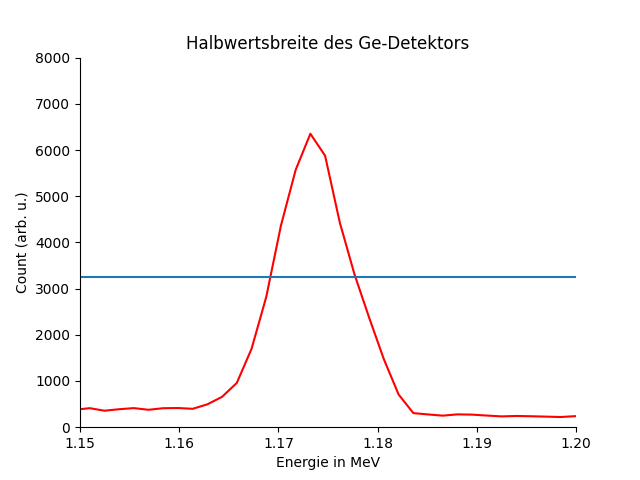
\includegraphics[width = \linewidth]{Bilder/Auswertung/Halbwertsbreite.png}
    \caption{Linienbreite der Cobalt-60 Quelle}
    \label{bild:linienbreite}
\end{figure}

Aus der Grafik \ref{bild:linienbreite} kann man herauslesen, dass die Halbwertsbreite circa 100keV. Die Energieauflösung ist circa die Hälfte der Halbwertsbreite. Das heißt 
die Energieauflösung ist ungefähr 50KeV, was vergleichbar ist mit der Auflösung eines NaJ-Szintillations-Detektor \cite[S.9]{Kador2021}. 

Außerdem sieht man an den Daten sehr schön die Comptonkanten. Dabei handelt es sich um Kanten im Spektrum, welche durch die Comptonstreuung entstehen. 
Da das Photon seinem 'Stoßpartner' aufgrund von Energie- und Impulserhaltung nur eine gewisse Potion Energie mitgeben kann, gibt es Oberkanten im 
Spektrum. Unterhalb der Kante kommt das Comptonkontinuum, welche Stöße mit Energieübertagung kleiner der maximalen Energiemenge sind.


\begin{figure}[ht]
    \centering
    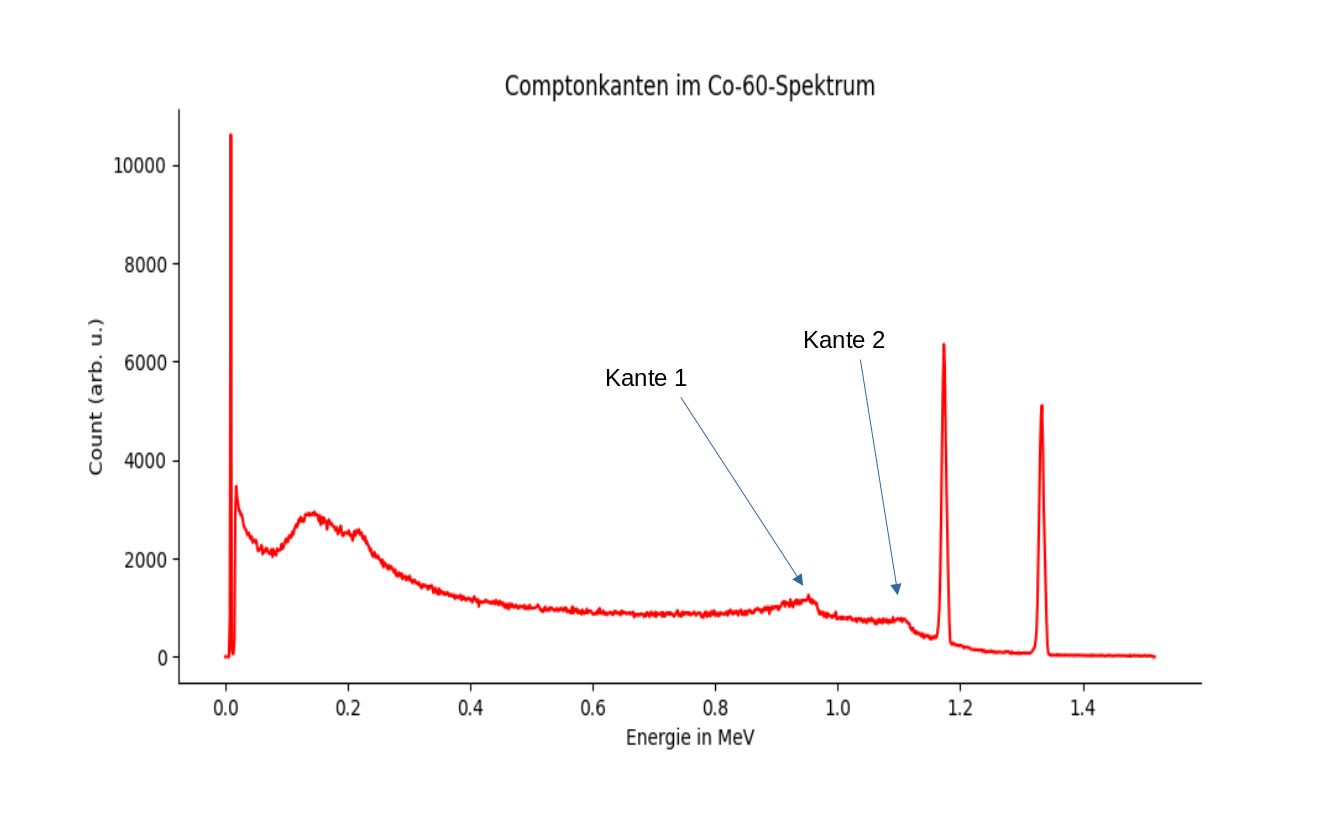
\includegraphics[width = \linewidth]{Bilder/Auswertung/Comtonkante.png}
    \caption{Comptonkanten: Kante 1 gehört zum Peak bei 1,2MeV, Kante zwei zum anderen Peak}
\end{figure}

\clearpage
